% -*- TeX -*- -*- DE -*-

\chapter{SimpleNet}\label{ch:SimpleNet}
\section{Einleitung}\label{sec:SimpleNet-Einleitung}
\textcolor{green}{\textit{Abgeschlossen: 27.10. v1}}\\
SimpleNet ist die zweite Methode, die im Rahmen dieser Arbeit genauer analysiert wird. Das am 28. März 2023 im Rahmen der Konferenz \ 
\glqq Computer Vision and Pattern Recognition\grqq{} veröffentlichte Paper \glqq SimpleNet: A Simple Network for Real-Time Instance Segmentation\grqq{} \
verspricht eine einfache, schnelle und präzise Methode. Es wird eine Genauigkeit von $\num{99,6}$\% AUROC auf MVTecAD bei einer 8-mal schnelleren Laufzeit im Vergleich zur \
PatchCore Variante, welche mit $\num{10}\%$ Subsampling in \ref{fig:patchcoreoriginal} zu sehen ist, propagiert. \ 
Es handelt sich also im Hiblick auf die Zielsetzung in dieser Arbeit um eine sehr vielversprechende Methode. \
\section{Funktionsweise}\label{sec:SimpleNet-Funktionsweise}
\textcolor{green}{\textit{Abgeschlossen: 27.10. v1}}\\
\begin{figure}[H]
    \centering
    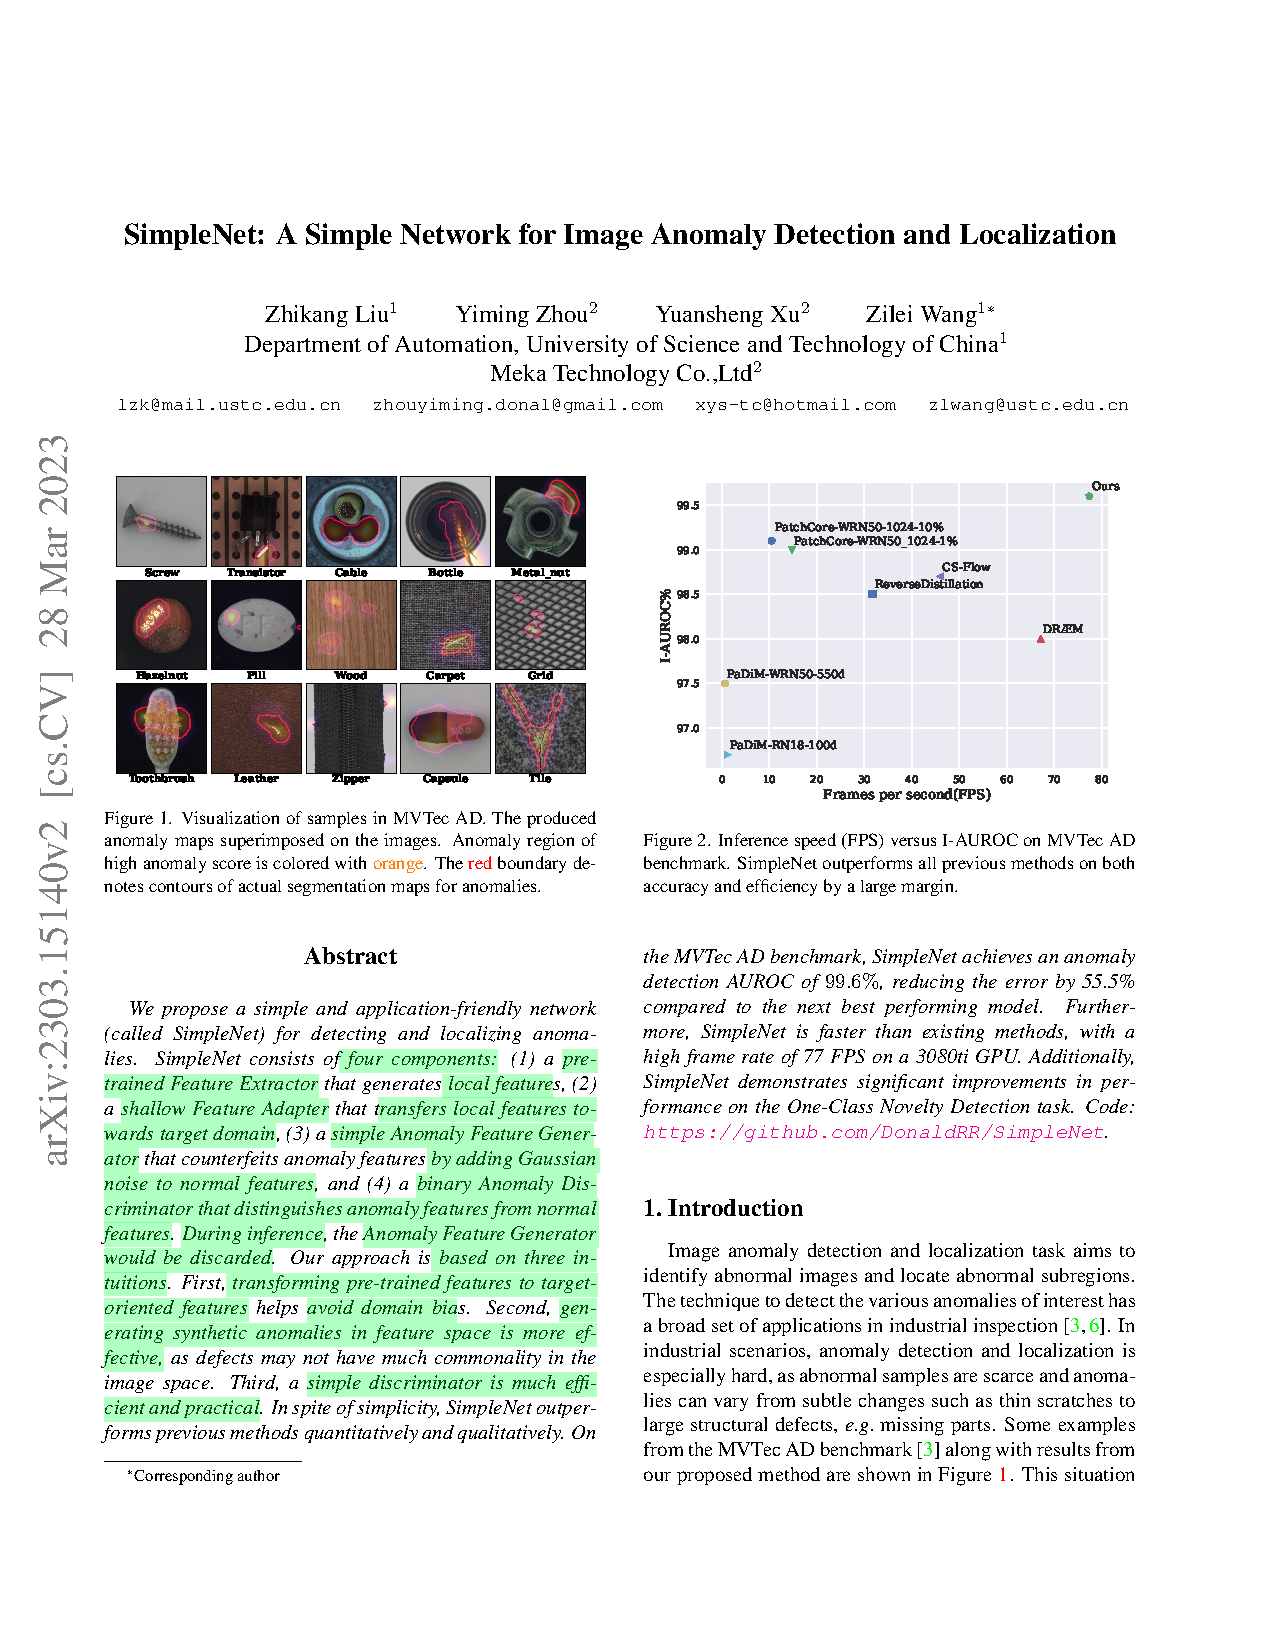
\includegraphics[width=0.8\textwidth]{bilder/SimpleNet.png}
    \caption{Funktionsweise von SimpleNet im Überblick \cite{SimpleNet}}
    \label{fig:simplenet}
\end{figure}
Die grobe Funktionsweise lässt sich anhand von Abbildung \ref{fig:simplenet} bereits gut erläutern. \
Analog zu den bisher vorgestellten Methoden muss auch hier zwischen einer Trainingsphase und der Inferenz- bzw. Testphase unterschieden werden. \
Die Teile der Abbildung, die mit gestrichelten Linien miteinander verbunden sind, werden nur während der Trainingsphase verwendet. \ 
Der obere Strang ist somit die Pipeline, die sequentiell während der Inferenz ausgeführt wird. \\
In der Trainingsphase werden nominale Bilder aus dem Trainingsdatensatz in einen vortrainierten \textbf{Feature Extraktor} gegeben - analog zu \ref{subsec:ErzeugenDerPatchFeatures}. \
Dessen Ausgabe wird dann in einem \textbf{Feature Adaptor} transformiert, um eine geeingetere Darstellung zu erhalten. \
Dann werden \textbf{Pseudo-Anomalien} aus den so entstandenen Feature erzeugt, indem zufällig Gauß'sches Rauschen aufaddiert wird. \
Schließlich wird ein \textbf{Diskriminator} trainiert, dessen Ziel es ist, diese Pseudo-Anomalien von nicht manipulierten und somit nominalen \
Feature zu unterscheiden. \\
Durch dieses Training wird der Diskriminator in die Lage versetzt, auch tatsächliche Anomalien zu erkennen. \\
Im Folgenden wird dieser Prozess schrittweise noch einmal genauer erläutert. \\
\subsection{Erzeugen der Patch Feature}\label{subsec:SimpleNet-FeatureExtraktor}
An dieser Stelle kann auf die Ausführungen in \ref{subsec:ErzeugenDerPatchFeatures} verwiesen werden. \ 
Der Prozess des Erzeugens von Patch Feature ist vollständig von der Methode PatchCore übernommen worden.\
Folglich gilt auch hier folgende Formel für die Menge aller Patch Feature, die aus einem Bild extrahiert werden: \\
$$
\mathcal{P}_{p}\left(\phi_{i,j}\right) = \left\{\phi_{i,j}\Big(\mathcal{N}_{p}^{(h,w)}\Big)| h\in\{1,...,h^{*}\}, w\in\{1,...,w^{*}\}\right\}
$$
mit der \glqq Neighborhood\grqq{} $\mathcal{N}_{p}^{h,w}$ und der Patchgröße $p$: \\
$$
\mathcal{N}_{p}^{h,w} = \left\{(a,b)| a \in \left[h-\left\lfloor \frac{p}{2}\right\rfloor,...,h+\left\lfloor \frac{p}{2} \right\rfloor\right], b \in \left[w-\left\lfloor \frac{p}{2}\right\rfloor,...,w+\left\lfloor \frac{p}{2}\right\rfloor\right]\right\}
$$
Dabei beizeichnet $i$ den Index des Eingagsbildes $x_{i}$, $j$ die Hierarchieebene des Feature Exktraktors $\phi$, welches ein vortrainiertes CNN ist. \
$h$ und $w$ geben die Ortskoordinate innerhalb einer Feature Map an, die die Größe $h^{*} \times w^{*}$ hat. \\
\subsection{Feature Adaptor}\label{subsec:SimpleNet-FeatureAdaptor}
Ein zusätzliches Element gegenüber PatchCore ist der Feature Adaptor $G_{\theta}$. \
Dieser hat die Aufgabe, die Patch Feature in eine kompaktere Darstellung zu überführen. \
Die Varianz der Patch Feature innerhalb einer Domäne wird dadurch reduziert, um besser in der Lage zu sein anomale Feature zu erkennen. \
Formal lässt sich der Feature Adaptor wie folgt beschreiben: \\
$$
G_{\theta}:\mathbb{R}^{c} \rightarrow \mathbb{R}^{c'}
$$
mit den Parametern $\theta$ und der Anzahl der Kanäle $c$ und $c'$. In der Veröffentlichung wurde konsequent $c = c'$ gewählt. \
Bei Versuchen zeigte sich, dass eine einfache lineare Transformation die besten Ergebnisse liefert. Es findet also eine Matrix-Vektor Multiplikation statt zwischen \ 
den einzelnen Patch Feature Vektoren $p_{h,w}$ aus $\mathcal{P}_{p}\left(\phi_{i,j}\right)$ und einer im Falle von $c = c'$ quadratischen Matrix $\theta$. \
Die so entstehenden Feature Vektoren $G_{\theta}(p_{h,w})$ werden im Folgenden als $q_{h,w}$ bezeichnet. \\
\subsection{Erzeugen der Pseudo-Anomalien}\label{subsec:SimpleNet-PseudoAnomalien}
Die Pseudo-Anomalien werden erzeugt, indem zufällig Gauß'sches Rauschen aufaddiert wird. \
$$
q_{h,w}^{-} = q_{h,w} + \epsilon, \epsilon \sim \mathcal{N}(\mu,\sigma^{2})
$$
Das Rauschen ist dabei unabhängig von den anderen Feature Vektoren (i.i.d.) und Mittelwertfrei ($\mu = 0$). \
Außerdem gilt naheliegenderweise $\epsilon \in \mathbb{R}^{c'}$. \
Durch Studie der offiziellen Implementierung werden weitere Details zu diesem Prozess deutlich. \
Aus einem Bild $x_{i}$ werden, wie bereits hinlänglich bekannt, die Patch Feature $\mathcal{P}_{p}\left(\phi_{i,j}\right)$ erzeugt. \
Für jeden dieser Patch Feature Vektoren $p_{h,w}$ wird jeweils ein zufälliger Vektor $\epsilon_{h,w}$ erzeugt und aufaddiert. \
Es wird also ein gesamtes Bild an Pseudo-Anomalien erzeugt. \
Dies unterscheidet sich von einer typischen strukturellen Anomalie, die nur einen kleinen Teil des Bildes betrifft. \
Weil aber jeder Patch Feature Vektor für sich genommen auf Anomalien geprüft wird und jedem einzelnen Patch Feature Vektor ein \
Anomliegrad zugeordnet wird, hat diese Abstraktion keinen negativen Einfluss auf die Ergebnisse. \
\subsection{Diskriminator}\label{subsec:SimpleNet-Diskriminator}
Der Diskriminator $D_{\psi}$ hat die Aufgabe, jedem einzelnen Patch Feature Vektor $q_{h,w}$ einen Anomaliegrad zuzuordnen. \
Negative Ausgaben deuten dabei auf Anomlien hin, während positive Ausgaben nominale Feature implizieren. \
Somit gilt, dass $D_{\psi}(q_{h,w}) \in \mathbb{R}$ ist. Es wurde hierfür ein einfaches, zweischichtiges Multi-Layer-Perzeptron verwendet. \
\subsection{Verlustfunktion und Training}\label{subsubsec:SimpleNet-Diskriminator-Verlustfunktion}
Der Disktiminator soll in die Lage versetzte werden, anomale Patch Feature Vektoren den Wert $th^{-}=\num{0,5}$ zuzordnen, während nominale Feature Vektoren \
den Wert $th^{+}=\num{0,5}$ erhalten sollen. \
Die Autoren verwenden dafür einen einfachen $l1$-Loss. Die Ausgabe wird auf positive Werte beschränkt. Es ergibt sich für ein Patch Feature Trainings-Tupel $(q^{i}_{h,w},q^{i-}_{h,w})$ \
folgende Verlustfunktion: \\
$$
l_{h,w}^{i}= \max \{0,th^{+}-D_{\psi}(q^{i}_{h,w})\} + \max \{0,D_{\psi}(q^{i-}_{h,w})-th^{-}\}
$$
Dieser Vorgang wird dann für alle Positionen $h$ und $w$ und über alle Bilder $x_{i}$ im Trainingsdatensatz $\mathcal{X}_{train}$ durchgeführt. \
Der Gesamtverlust ergibt sich dann aus der Summe aller Verluste: \\
$$
\mathcal{L} = \sum_{x_{i}\in\mathcal{X}_{train}} \sum_{h,w} \frac{l_{h,w}^{i}}{w^{*}h^{*}}
$$
Dabei gilt $(h,w)\in\{1,...,h^{*}\}\times\{1,...,w^{*}\}$. Diese Funktion wird minimiert im Sinne der Parameter $\theta$ und $\psi$. \
Das bedeutet, dass sowohl der Feature Adaptor $G_{\theta}$ als auch der Diskriminator $D_{\psi}$ trainiert werden. 
\subsection{Bestimmen des Anomaliegrades (Inferenz)}\label{subsec:SimpleNet-Inferenz}
Wie bereits erwähnt, wird bei der Inferenz ein Bild $x_{i}$ in Patch Feature $\mathcal{P}_{p}\left(\phi_{i,j}\right)$ überführt. \
Diese werden dann in den Feature Adaptor gegeben, um die Feature Vektoren $q_{h,w}$ zu erhalten. \
Abschließend werden diese Feature Vektoren in den Diskriminator gegeben, um den Anomaliegrad $s_{h,w}=D_{\psi}(q_{h,w})$ zu erhalten. \
So kann dann durch das Zusammenführen der räumlichen Information die Anomaliekarte für das gesamte Bild bestimmt werden. \
Für diese Arbeit relevant ist aber vor allem der Anomliegrad des gesamten Bildes. Dies geschieht einfach über die Maximalwertbildung über die Anomaliekarte. \
$$
s_{i} = \max_{h,w} s_{h,w}
$$
Abschließend wird, wie bereits bekannt, der AUROC über den gesamten Testdatensatz berechnet. \\
\section{Ergebnisse und Diskussion der Originalmethde}\label{sec:SimpleNet-ErgebnisseUndDiskussion}
\textcolor{green}{\textit{Abgeschlossen: 01.11. v1}}\\
Wie bereits in der Einleitung erwähnt, sind die Ergebnisse der Veröffentlichung sehr vielversprechend. \
Die Ergebnisse konnten zum größten Teil auch reproduziert werden. \\
Mit einem AUROC von $\num{99,6}$\% auf MVTecAD ist die Methode sehr präzise. \
Für dieses Ergebnis ist allerdings ein \glqq Early Stopping\grqq{} notwendig, was kritisch hinterfragt werden sollte. \
Es ist durchaus der Fall, dass ein fallender Verlust mit einer gesteigerten Genauigkeit einhergeht. Diese starke Korrelation ist aber nicht immer gegeben. \
Es ist also nicht zwingend der Fall, dass ein fallender Verlust auch zu einer gesteigerten Genauigkeit führt. \ 
In vielen Fällen ist die höchste, während des Trainings erreichte Genauigkeit, nicht die, die am Ende des Trainings erreicht wird. \\
In der Originalimplementierung ist ein Training über 40 Epochen vorgesehen, was bedeutet, dass der Trainigsdatensatz $\mathcal{X}_{train}$ 40 mal durchlaufen wird. \
Nach jeder dieser Epochen wird das das Modell nicht etwa auf einem Validierungsdatensatz getestet, sondern auf dem gesamten Testdatensatz. \
Das Modell, welches die höchste Genauigkeit erreicht, wird dann gespeichert und für die finale Inferenz, also die Berechnung des AUROC, verwendet. \
Dieses Vorgehen ist fragwürdig, weil der Testdatensatz für solche Zwecke nicht vorgesehen ist. \
In der Realität steht ein solcher Testdatensatz, der dann zum Beispiel einer produktiven Produktion entspricht, nicht zur Verfügung. \
Dieses Problem wird zu späterer Stelle noch einmal aufgegriffen. \\
Mit Hinblick auf die Laufzeit ist die Methode für eine Inferenz ohne GPU wohl kaum schneller als die Methode PatchCore. \
Ein Unterschied in der Laufzeit kann nur bei den Bausteinen erzeugt werden, die überhaupt unterschiedlich sind. \
Um eine gegenüber PatchCore gerinigere Laufzeit zu erreichen, muss also der Feature Adaptor oder der Diskriminator schneller sein, \
als die NN-Suche und das wenig zeitkritische Berechnen des Anomaliegrades. \ Berachtet man die Ergebnisse der PatchCore Methode, \
so ist die Laufzeit der NN-Suche und des Berechnens des Anomaliegrades im Verhältnis sehr gering. \
Es ist also kaum zu erwarten, dass signifikante Verbesserungen in der Laufzeit gegenüber PatchCore erreicht werden können. \
Dass die Autoren darauf verweisen, ihre Methode sei 8-mal schneller als PatchCore, ist nur vor dem Hintergrund der Verwendung einer GPU zu verstehen. \
Die Methode SimpleNet kann komplett mithilfe einer GPU ausgeführt werden, weil nur bekannte Feed-Forward-Operationen verwendet werden (CNN, MLP). \
Weil sich allerdings auch die NN-Suche durch eine GPU enorm beschleunigen würde, worauf auch die Autoren von PatchCore bereits hinwiesen, \
und in keiner der Versuche zu PatchCore die NN-Suche der laufzeitkritischste Teil war, ist die Aussage der Autoren von SimpleNet für den Autor nur schwer nachvollziehbar. \\
Die Methode ist dennoch spannend, weil sie sich nicht nur durch einen tatsächlich sehr einfachen Aufbau auszeichnet, sondern auch Potentiale für weitere Forschung bietet. \
So ist zum Beispiel denkbar, dass durch ein spezifischeres Design der Pseudo-Anomalien, die Ergebnisse noch weiter verbessert werden können. \
In jedem Fall liefert SimpleNet den Beweis, dass ein solches Vorgehen prinzipiell funktioniert. \\